% !TeX TS-program = luatex

\documentclass[11pt, aspectratio=169]{beamer}

\usetheme{Antibes}
\usecolortheme{seahorse}
\setbeamertemplate{navigation symbols}{}
\setbeamertemplate{headline}{}
\graphicspath{ {./images/} }

% Fonts and emojis
\usepackage{emoji}
\usepackage{fontspec}
\setsansfont{Fira Sans}
\setmonofont{Iosevka}
\usepackage{ulem}

% Codeblocks
\usepackage{minted}
\usemintedstyle{monokai}

% Links coloring
\usepackage{hyperref}
\hypersetup{
	colorlinks=true,
	linkcolor=blue,
	filecolor=magenta,
	urlcolor=blue,
}

\title[Building Helm replacement]{Building Helm replacement:\\from templating strings to populating objects}
\author{Denis Shatokhin}
\date{September 2024}

\begin{document}
\maketitle

\begin{frame}{\emoji{card-index-dividers} Table of Content}
	\tableofcontents
\end{frame}

\section{Introduction}

\begin{frame}{\emoji{waving-hand} About Me}
	\begin{description}
		\item [$\bullet$ Devops Engineer (System Administrator)]
		\item [$\bullet$ Work at Relex Solutions]
		\item [$\bullet$ Live in Helsinki for almost 2 years]
		\item [$\bullet$ Really like to build solutions no one asked for]
	\end{description}
\end{frame}

\begin{frame}{\emoji{warning} Disclaimer}
	\textbf{Helm} is a great tool and you should use it.\\~\\
	All what I'm about to show is just artifacts of my learning process.\\~\\
	I just would like to share my ideas with you\\~\\

	\centerline{{\Huge \emoji{smiling-face-with-smiling-eyes}}}
\end{frame}

\section{Helm and it's drawbacks}

\begin{frame}{\emoji{scroll} History of Helm}
	Originally \textbf{Helm} was presented in 2015 on the KubeCon,
	in 2016 project was merged with Kubernetes Deployment Manager,
	this is how \textbf{Helm 2} was born which contained 2 components -
	\textbf{Helm} itself as a client and \textbf{Tiller} as a server.\\~\\
	\textbf{Helm 3} was released in 2019 and this what we use and love today\\~\\
	Source: \href{https://helm.sh/docs/community/history}{helm.sh/docs/community/history}\\~\\

	\centerline{{\Huge \emoji{heart}}}
\end{frame}

\begin{frame}[fragile]{\emoji{package} Helm Charts}
	Helm chart contains templates, metadata and defaults for rendering and applying
	kubernetes manifests.

	Usually it's just a gzip archive, which directory structure looks like this:

	\begin{minted}[bgcolor=gray,fontsize=\small]{text}
├── Chart.yaml
├── templates
│   ├── deployment.yaml
│   ├── _helpers.tpl
│   ├── hpa.yaml
│   ├── ingress.yaml
│   ├── NOTES.txt
│   ├── serviceaccount.yaml
│   └── service.yaml
└── values.yaml
	\end{minted}
\end{frame}

\begin{frame}[fragile]{\emoji{receipt} Metadata}
	A \textbf{Chart.yaml} file contains some metadata, such as name, description,
	version, version of the application to be deployd etc.
	\begin{minted}[bgcolor=darkgray]{Yaml}
# Chart.yaml
apiVersion: v2
name: chart
description: A Helm chart for Kubernetes
type: application

version: 0.1.0

appVersion: "1.16.0"
	\end{minted}
\end{frame}

\begin{frame}[fragile]{\emoji{page-facing-up} Manifests Templates}
	Just a regular Golang templates
	\begin{minted}[bgcolor=darkgray]{Yaml}
# templates/serviceaccount.yaml
{{- if .Values.serviceAccount.create -}}
apiVersion: v1
kind: ServiceAccount
metadata:
  name: {{ include "chart.serviceAccountName" . }}
  labels:
    {{- include "chart.labels" . | nindent 4 }}
  {{- with .Values.serviceAccount.annotations }}
  annotations:
    {{- toYaml . | nindent 4 }}
  {{- end }}
automountServiceAccountToken: {{ .Values.serviceAccount.automount }}
{{- end }}
	\end{minted}
\end{frame}

\begin{frame}[fragile]{\emoji{raising-hands} Helpers}
	Helpers are defined functions to reuse in templates
	\begin{minted}[bgcolor=darkgray,fontsize=\small]{Smarty}
{{/*
templates/_helpers.tpl
*/}}
{{- define "chart.serviceAccountName" -}}
  {{- if .Values.serviceAccount.create }}
    {{- default (include "chart.fullname" .) .Values.serviceAccount.name }}
  {{- else }}
    {{- default "default" .Values.serviceAccount.name }}
  {{- end }}
{{- end }}
	\end{minted}
\end{frame}

\begin{frame}[fragile]{\emoji{writing-hand} Values}
	Values contains default values for templating manifests,
	here is service account section
	\begin{minted}[bgcolor=darkgray]{Yaml}
# values.yaml
serviceAccount:
  create: true
  automount: true
  annotations: {}
  name: ""
	\end{minted}
\end{frame}

\begin{frame}[fragile]{\emoji{hammer} The Misuse of YAML \emoji{nut-and-bolt} }
	According to \href{https://yaml.org}{yaml.org}:
	\begin{minted}[bgcolor=darkgray]{Yaml}
%YAML 1.2
---
YAML: YAML Ain't Markup Language™

What It Is:
  YAML is a human-friendly data serialization
  language for all programming languages.
    \end{minted}

	So why are we even trying to template 'human-friendly' text file
	before sending it to the Kubernetes API?\\~\\
	\centerline{{\Huge \emoji{thinking-face}}}
\end{frame}

\section{My solution (with it's own drawbacks)}

\begin{frame}[fragile]{\emoji{light-bulb} The Idea}
	\emoji{stop-sign} Stop templating strings\\~\\
	\emoji{rocket} Let's populate typed objects with values\\~\\

	We may use some recently opensourced configuration language\\~\\
	\centerline{{\Huge \emoji{red-apple} \emoji{cucumber}}}
\end{frame}

\begin{frame}{\emoji{sparkles} Introducing Pelm}
	\textbf{Pelm} is high level and type aware \sout{package manager} \textbf{Helm} clone.\\~\\
	Under the hood it's using \href{https://pkl-lang.org}{Apple PKL} for constructing Kubernetes manifests.\\~\\
\end{frame}

\begin{frame}{\emoji{cucumber} Apple Pkl}
	\textit{pronounced Pickle}\\~\\
	Build by Apple and open-sourced earlier this year:

	\begin{block}{quote}
		Pkl -- is an embeddable configuration language which provides rich support
		for data templating and validation. It can be used from the command line,
		integrated in a build pipeline, or embedded in a program. Pkl scales
		from small to large, simple to complex, ad-hoc to repetitive configuration tasks.
	\end{block}

	\begin{description}
		\item [$\bullet$ turing complete]
		\item [$\bullet$ written in java]
		\item [$\bullet$ LSP support on the corner]
		\item [$\bullet$ community growing fast]
	\end{description}
\end{frame}

\begin{frame}{\emoji{label} Why it's called PELM}
	Since \textbf{pkl-lang} is used I've changed the first letter:\\~\\
	\centerline{{\Huge HELM -> PELM}}\\

	This is exactly what you'd get instead of \textbf{Helm} if it was downloaded from a scatchy web site\\~\\
\end{frame}

\begin{frame}{\emoji{dumpling} Because of PELMENI}
	\begin{columns}
		\column{0.4\textwidth}
		Remembers me about \textbf{PELMENI}\\~\\
		\centerline{{\Huge \emoji{face-savoring-food}}}

		\column{0.6\textwidth}
		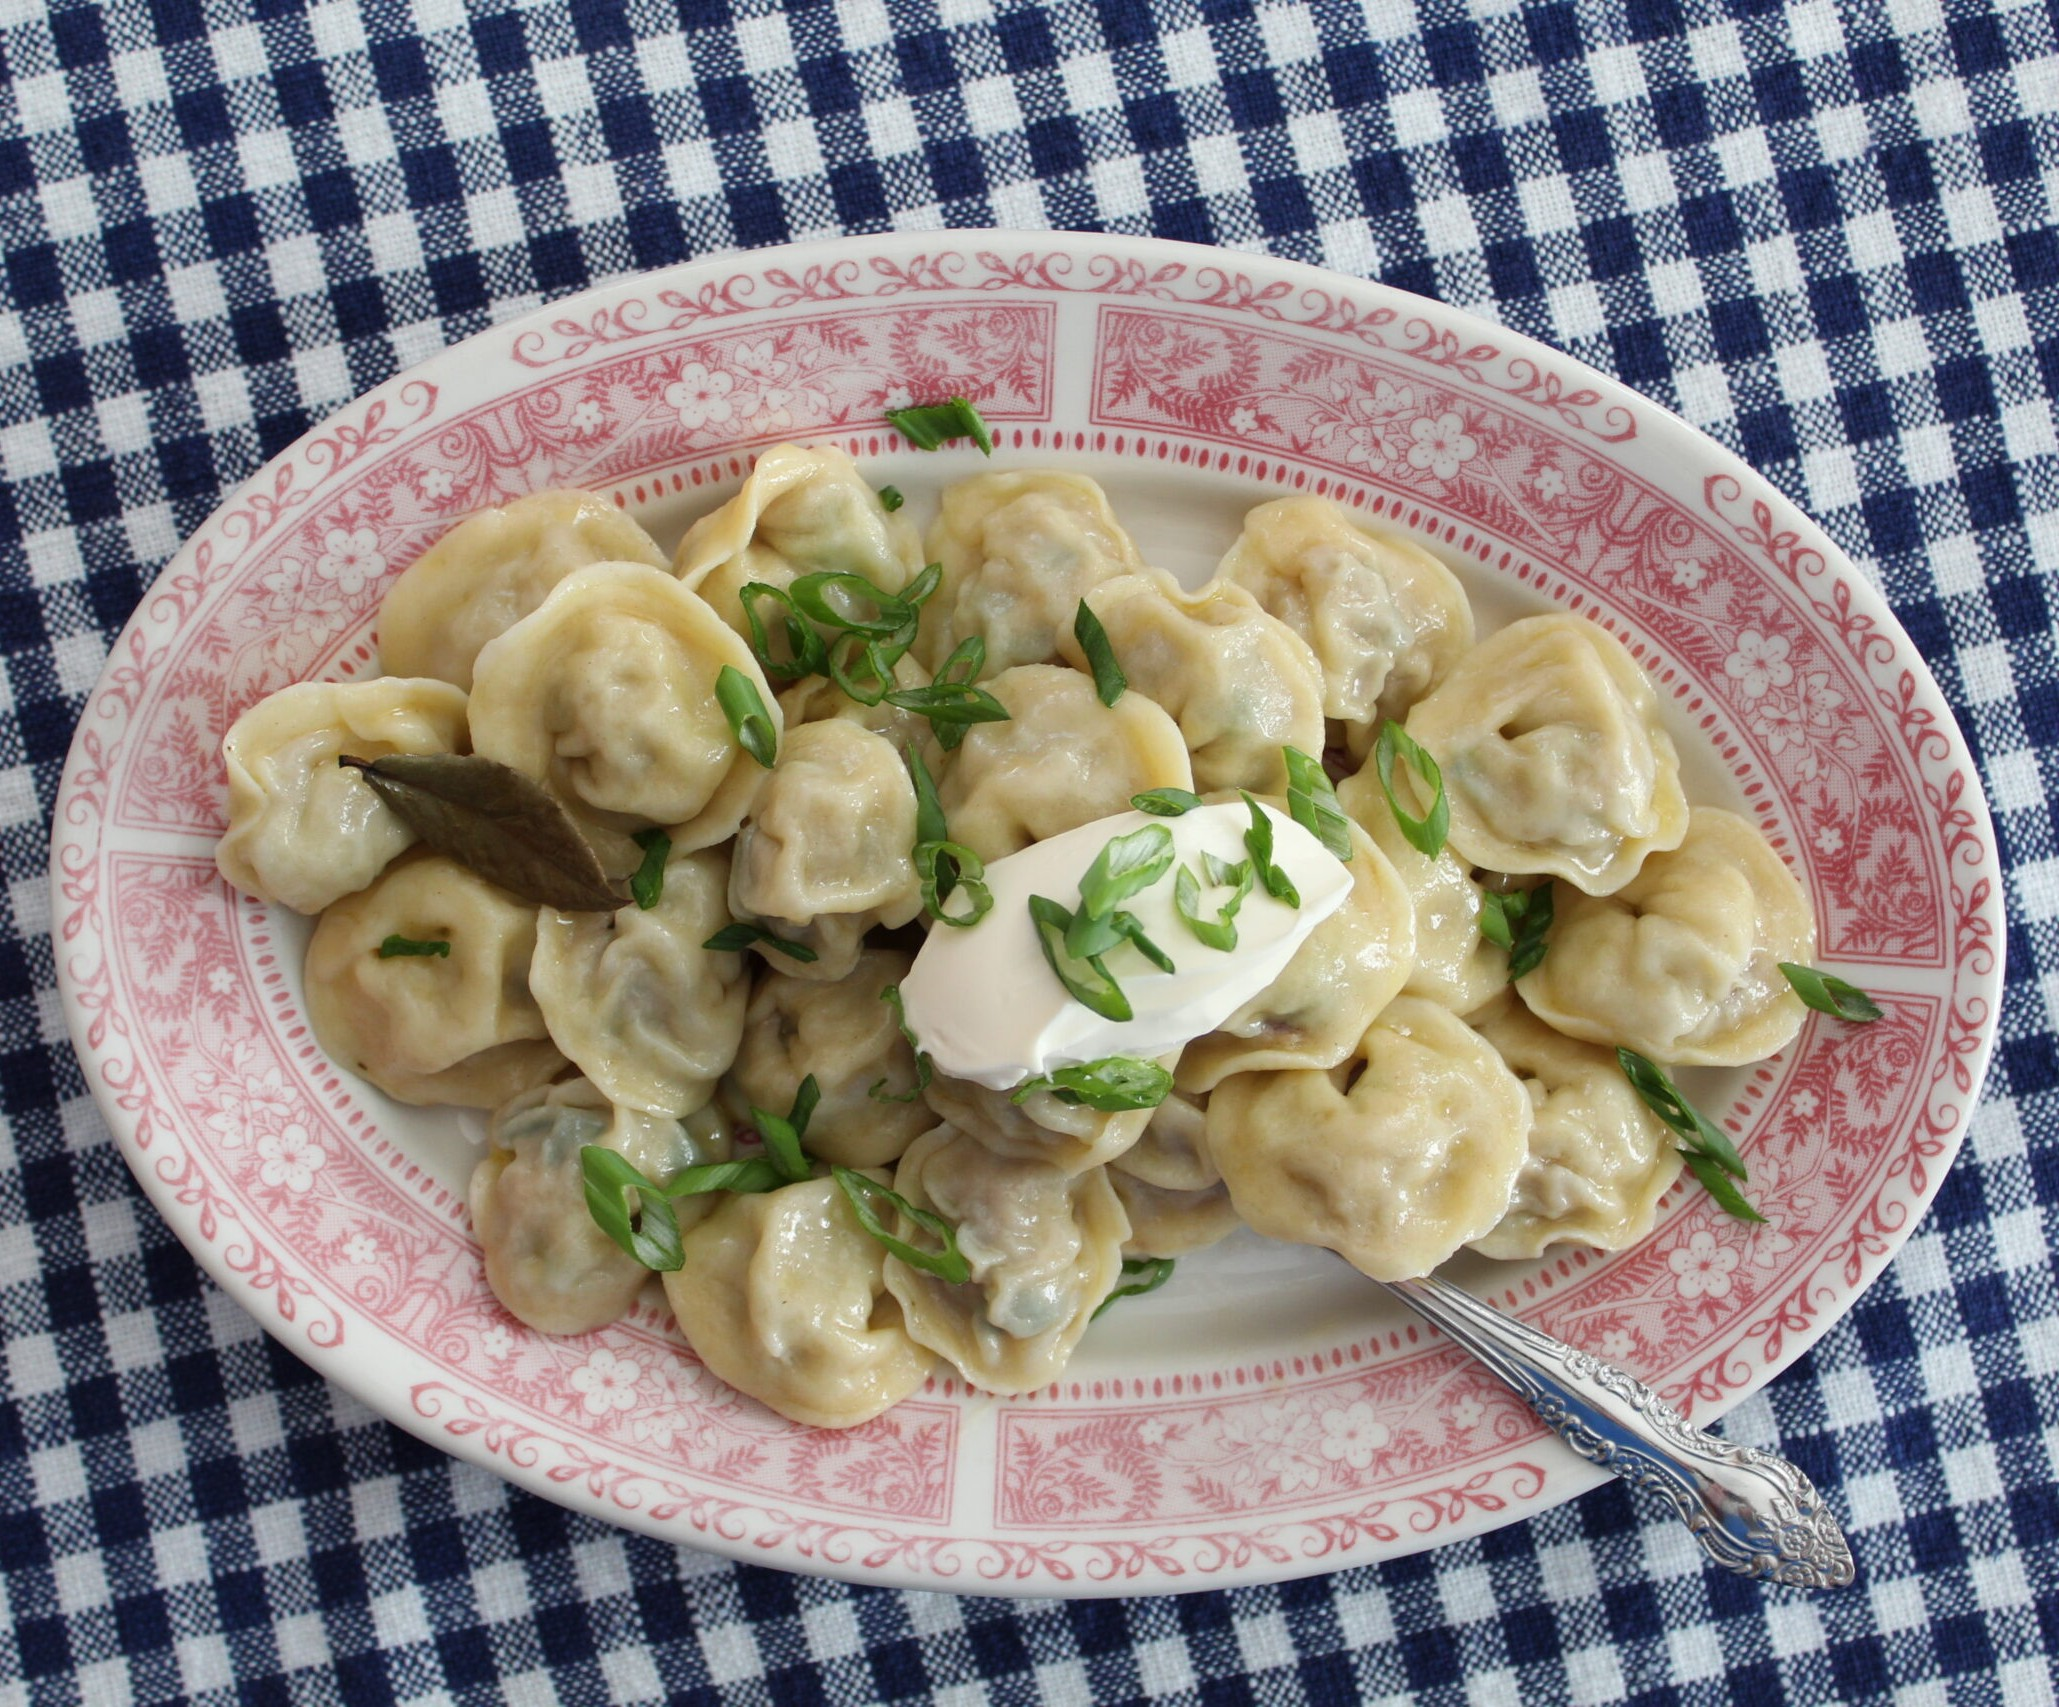
\includegraphics[width=\textwidth]{pelmeni.jpeg}
	\end{columns}
\end{frame}
% dumpling
\begin{frame}[fragile]{\emoji{canned-food} Pelm Jars}
	\textit{Almost} the same as \textbf{Helm Charts}
	\begin{minted}[bgcolor=gray,fontsize=\small]{Text}
├── helpers.pkl
├── jar.pkl
├── pelm.pkl
├── PklProject
├── renderer.pkl
├── templates
│   ├── deployment.pkl
│   ├── hpa.pkl
│   ├── ingress.pkl
│   ├── serviceaccount.pkl
│   └── service.pkl
└── values.pkl
	\end{minted}
\end{frame}

\begin{frame}[fragile]{\emoji{receipt} Pelm Metadata}
	A \textbf{jar.pkl} file contains almost identical to \textbf{Chart.yaml} metadata
	\begin{minted}[bgcolor=darkgray]{Kotlin}
// jar.pkl
name = "kuard"

description = "A Pelm jar for Kubernetes"

version = "0.1.0"

appVersion = "1.27.1"
	\end{minted}
\end{frame}

\begin{frame}[fragile]{\emoji{page-facing-up} Pelm Manifests}
	\begin{minted}[bgcolor=darkgray,fontsize=\small]{Kotlin}
// templates/serviceaccount.pkl
import "@k8s/api/core/v1/ServiceAccount.pkl"
import ".../pelm.pkl"

manifest: ServiceAccount? = if (pelm.values.serviceAccount.create) new {
  metadata {
    name = pelm.helpers.serviceAccountName
    namespace = pelm.namespace
    labels = pelm.helpers.labels
    annotations = pelm.values.serviceAccount.annotations
  }
  automountServiceAccountToken = pelm.values.serviceAccount.automount
} else null
	\end{minted}
\end{frame}

\begin{frame}[fragile]{\emoji{raising-hands} Pelm Helpers}
	Helpers are defined functions to reuse in templates
	\begin{minted}[bgcolor=darkgray]{Kotlin}
// helpers.pkl
serviceAccountName: String =
  if (values.serviceAccount.create)
    values.serviceAccount.name ?? fullname
  else
    values.serviceAccount.name ?? "default"
	\end{minted}
\end{frame}

\begin{frame}[fragile]{\emoji{writing-hand} Pelm Values}
	Default values stored in \textbf{values.pkl}, and the overrides can be
	provided as an additional \textbf{values.yaml} file
	(the same service account section)

	\begin{columns}
		\column{0.5\textwidth}
		\begin{minted}[bgcolor=darkgray]{Kotlin}
// values.pkl
defaultValues = new Values {
  serviceAccount = new {
    create = true
    automount = true
    annotations = new {}
    name = null
  }
}
		\end{minted}

		\column{0.5\textwidth}
		\begin{minted}[bgcolor=darkgray]{Yaml}
# values.yaml
serviceAccount:
  create: true
  automount: true
  annotations: {}
  name: ""
		\end{minted}
	\end{columns}
\end{frame}

\begin{frame}{\emoji{balance-scale} Comparison to other tools}
	Well, not a lot to compate to, actually.
	\textbf{Helm} has 9 years of active development,
	\textbf{Kustomize} has opposite stratagy with patches.\\~\\
	There is also \href{https://github.com/kptdev/kpt}{KPT} created by
	\href{https://github.com/bgrant0607}{Brian Grant}
	(lead architect of Kubernetes which created kubectl apply and kustomize),
	but it is covering the deployment from top to bottom.\\~\\
	\textbf{Pelm} on the other hand, have the same mechanics as \textbf{Helm},
	but different templating engine.
\end{frame}

\section{Demo}

\begin{frame}{\emoji{crossed-fingers} Demo}
	Let's create a \textbf{Pelm Jar}, change it according to our needs
	and deploy it to fresh Kubernetes cluster\\~\\
	\centerline{{\Huge \emoji{smirking-face}}}
\end{frame}

\begin{frame}{\emoji{person-shrugging} Pelm's Drawbacks}
	\begin{description}
		\item [$\bullet$ Lacking prune capabilities]
		\item [$\bullet$ Complex logic in templates can ruin the fun]
		\item [$\bullet$ No registries (OCI or jar museum)]
		\item [$\bullet$ Written in Javascript]
		\item [$\bullet$ Probably only working on my machine]
	\end{description}
\end{frame}

\section{Questions}

\begin{frame}{\emoji{link} Links}
	Code and presentation:
	\begin{description}
		\item [$\bullet$ \href{https://github.com/dshatokhin/pelm}{github.com/dshatokhin/pelm}]
		\item [$\bullet$ \href{https://github.com/dshatokhin/presentations}{github.com/dshatokhin/presentations}]
	\end{description}~

	Additional links:
	\begin{description}
		\item [$\bullet$ \href{https://github.com/pkl-community/awesome-pkl}{github.com/pkl-community/awesome-pkl}
		      -- Awesome Pkl]
		\item [$\bullet$ \href{https://github.com/apple/pkl/issues/354}{github.com/apple/pkl/issues/354}
		      -- Support OCI registries for Pkl packages]
		\item [$\bullet$ \href{https://github.com/helm/helm/issues/12780}{github.com/helm/helm/issues/12780}
		      -- Adopt Pkl for Helm]
		\item [$\bullet$ \href{https://github.com/MarkSRobinson/nginx-pkl}{github.com/MarkSRobinson/nginx-pkl}
		      -- NGINX Pkl Chart]
	\end{description}
\end{frame}

\begin{frame}{\emoji{red-question-mark} Questions}
	If you have any...
\end{frame}
\end{document}
